\documentclass[11pt,a4paper]{article}

\usepackage[utf8]{inputenc}
\usepackage[T1]{fontenc}
\usepackage[spanish]{babel}
\usepackage{geometry}
\usepackage{array}
\usepackage{longtable}
\usepackage{booktabs}
\usepackage{tabularx}
\usepackage{hyperref}
\usepackage{enumitem}
\usepackage{graphicx}
\graphicspath{{../figures/}}
\usepackage{float}
\usepackage{amsmath}

\geometry{top=2.5cm,bottom=2.5cm,left=2.5cm,right=2.5cm}
\hypersetup{
	colorlinks=true,
	linkcolor=blue,
	urlcolor=blue,
	pdftitle={Elección del dataset},
	pdfauthor={Grupo de trabajo}
}

\renewcommand{\arraystretch}{1.15}
\setlength{\parindent}{0pt}
\setlength{\parskip}{0.65em}
\setlength{\emergencystretch}{2em}

\title{\textbf{Trabajo Final - Grupo 1}}
\author{Matías López, Isidro Silicaro Pera, Taciano Pacchialat}
\date{}

\begin{document}

\maketitle

\section{Introducción al dominio: ¿Qué es la UFC?}

La \textbf{UFC} (\textit{Ultimate Fighting Championship}) es la organización de artes marciales mixtas (MMA, por sus siglas en inglés) más grande e importante del mundo. Las MMA son un deporte de combate que permite a los atletas utilizar técnicas de múltiples disciplinas marciales: golpeo de pie (como el boxeo o el kickboxing), lucha en pie (como el judo o la lucha olímpica) y combate en el suelo (como el jiu-jitsu brasileño o el wrestling).

\subsection*{Estructura de una pelea}

Cada enfrentamiento tiene lugar en un área de combate octagonal denominada \textbf{octágono}, con dos competidores ubicados en los llamados \textbf{rincón rojo} y \textbf{rincón azul}. Una pelea se divide en \textbf{rounds} (asaltos) de cinco minutos cada uno. Las peleas regulares constan de tres rounds; las disputas por un \textbf{título} (campeonato de una categoría de peso) se extienden a cinco rounds.

Una pelea puede finalizar de las siguientes maneras:

\begin{itemize}[leftmargin=*]
  \item \textbf{Nocaut (KO):} Un competidor derriba al otro y este queda inconsciente o sin capacidad de continuar.
  \item \textbf{Nocaut técnico (TKO):} El árbitro detiene la pelea porque uno de los peleadores no puede defenderse adecuadamente, aunque no haya perdido el conocimiento.
  \item \textbf{Sumisión (Submission):} Un competidor aplica una llave articular o una estrangulación y el rival da un golpecito en señal de rendición (\textit{tapout}), o bien el árbitro para la pelea al advertir que el afectado está inconsciente.
  \item \textbf{Decisión de los jueces (Decision):} Si ninguno finaliza la pelea antes del límite de tiempo, tres jueces puntúan los rounds y determinan al ganador. Puede ser unánime, dividida o por mayoría.
  \item \textbf{Descalificación o No Contest:} Situaciones menos frecuentes por infracciones graves o accidentes.
\end{itemize}

\subsection*{Categorías de peso}

Los peleadores compiten dentro de \textbf{divisiones de peso} (por ejemplo, Strawweight, Flyweight, Bantamweight, Featherweight, Lightweight, Welterweight, Middleweight, Light Heavyweight, Heavyweight), lo que asegura que los competidores sean físicamente comparables entre sí. Cada división tiene su propio campeón.

\subsection*{Métricas estadísticas de combate}

Durante cada pelea se registran numerosas estadísticas. A continuación se define el vocabulario técnico utilizado en el dataset:

\begin{itemize}[leftmargin=*]
  \item \textbf{Golpe significativo (\textit{significant strike}):} Golpe de puño, patada, rodillazo o codazo considerado de suficiente impacto para ser contabilizado. Excluye golpes superficiales o de baja intensidad.
  \item \textbf{Golpe total (\textit{total strike}):} Cualquier golpe intentado o conectado, incluyendo golpes de menor impacto que los significativos.
  \item \textbf{Precisión (\textit{accuracy}):} Proporción de golpes o derribos conectados sobre el total de intentos, expresada en porcentaje.
  \item \textbf{Derribo (\textit{takedown}):} Acción de llevar al rival al suelo mediante técnicas de lucha.
  \item \textbf{Defensa de derribo (\textit{takedown defense}):} Porcentaje de intentos de derribo del rival que se logran neutralizar.
  \item \textbf{Control (\textit{ctrl}):} Tiempo (en segundos) que un peleador domina a su rival en el suelo, en una posición de ventaja.
  \item \textbf{Intento de sumisión (\textit{submission attempt}):} Cantidad de veces que un peleador intenta aplicar una llave o estrangulación durante la pelea.
  \item \textbf{Knockdown (KD):} Evento en que un competidor envía al suelo a su rival con un golpe, aunque este puede levantarse y continuar.
  \item \textbf{Golpeo por zona (\textit{head / body / leg}):} Estadísticas separadas de golpes dirigidos a la cabeza, al torso o a las piernas.
  \item \textbf{Golpeo por distancia (\textit{distance / clinch / ground}):} Estadísticas separadas según la fase del combate: larga distancia (intercambio de pie), clinch (cuerpo a cuerpo de pie) o suelo (grappling en el piso).
  \item \textbf{SLpM (\textit{Significant Strikes Landed per Minute}):} Promedio histórico de golpes significativos conectados por minuto.
  \item \textbf{SApM (\textit{Significant Strikes Absorbed per Minute}):} Promedio histórico de golpes significativos recibidos por minuto, indicador de cuánto daño absorbe un peleador.
  \item \textbf{Defensa de golpes (\textit{str\_def}):} Porcentaje de golpes significativos del rival que se logran esquivar o bloquear.
  \item \textbf{Postura (\textit{stance}):} Posición de combate del peleador: \textit{Orthodox} (zurda derecha adelante), \textit{Southpaw} (zurdo con la izquierda adelante) u otras variantes.
  \item \textbf{Reach (envergadura):} Distancia en pulgadas entre los extremos de ambas manos con los brazos extendidos horizontalmente; a mayor reach, mayor distancia de golpeo efectiva.
\end{itemize}

\section{Descripción general del dataset}

En este trabajo se utilizará el conjunto de datos \textit{UFC Datasets 1994-2025}, disponible en Kaggle bajo el nombre \url{https://www.kaggle.com/datasets/neelagiriaditya/ufc-datasets-1994-2025}.

El dataset fue seleccionado porque agrupa de manera detallada el historial de peleas de la UFC, sus atributos físicos, técnicas y resultados de los combates a lo largo de más de 30 años. Esta información presenta una oportunidad muy valiosa para realizar tareas de análisis de datos, estudiar las evoluciones de estilos de pelea, examinar estadísticas entre peleadores y estimar probabilidades sobre resultados de combates.

El objetivo del trabajo es construir conocimiento descriptivo y probabilístico a partir de la información histórica para apoyar decisiones en escenarios de combate y entrenamiento.

En particular, se busca responder preguntas como las siguientes:

\begin{itemize}[leftmargin=*]
\item ¿Qué luchador tiene mayor probabilidad de ganar una pelea dada?
\item Si soy un luchador con determinadas características, ¿qué tipo de pelea me conviene aceptar?
\item Si soy una persona con determinadas características, ¿qué estilo me conviene practicar?
\end{itemize}

\section{Origen y características generales}

El conjunto de datos unificado \path{UFC.csv} disponible como parte de los datasets de UFC contiene \textbf{8.337 registros} y \textbf{124 columnas}. Reúne una vasta cantidad de atributos capturados a lo largo de décadas mostrando un detallado registro por cada pelea que ocurrió en diversas locaciones del mundo a partir de 1994 hasta inicios de 2025. 

De manera general, el conjunto de datos clasifica su información en las siguientes partes:

\begin{itemize}[leftmargin=*]
	\item \textbf{Variables de contexto de evento:} nombre del evento, fecha, locación y división de peso.
	\item \textbf{Variables del combate:} tiempo total de combate, si es o no por el título, y método de finalización (sumisión, nocaut, decisión, etc.).
	\item \textbf{Variables específicas por rincón (Rojo \texttt{r\_} y Azul \texttt{b\_}):} información recolectada del peleador antes y durante el combate, que abarca desde la edad, postura y dimensiones físicas, hasta métricas clave de desempeño como precisión de los golpes, intentos de derribo, control en el suelo, y otros tipos de agresiones.
	\item \textbf{Variables de salida:} resultado observado de la pelea indicando quién fue el vencedor del enfrentamiento.
\end{itemize}

Los datos fueron relevados haciendo un scraping del sitio \url{http://ufcstats.com/statistics/events/completed}.

\section{Descripción completa de las columnas}

Dado el gran número de dimensiones (124), se describe la totalidad de columnas del archivo \path{UFC.csv} agrupándolas por su función analítica. La columna \textbf{Tipo} indica el tipo de dato predominante: \textit{str} (cadena de texto), \textit{int} (entero), \textit{float} (numérico con decimales), \textit{date} (fecha), \textit{bool} (booleano) y \textit{cat} (variable categórica).

\small
\begin{longtable}{>{\raggedright\arraybackslash}p{5.6cm}>{\raggedright\arraybackslash}p{1.3cm}>{\raggedright\arraybackslash}p{5.1cm}}
\caption{Cobertura completa de columnas del dataset UFC (124 columnas).}\label{tab:variables}\\
\toprule
\textbf{Columnas incluidas} & \textbf{Tipo} & \textbf{Descripción} \\
\midrule
\endfirsthead

\toprule
\textbf{Columnas incluidas} & \textbf{Tipo} & \textbf{Descripción} \\
\midrule
\endhead

\bottomrule
\endfoot

\path{event_id} & \textit{str} & Identificador único del evento. \\
\path{event_name} & \textit{str} & Nombre oficial del evento (ej.\ ``UFC 300''). \\
\path{date} & \textit{date} & Fecha de realización del evento. \\
\path{location} & \textit{str} & Ciudad y país donde se celebró el evento. \\
\path{fight_id} & \textit{str} & Identificador único de la pelea. \\
\path{division} & \textit{cat} & Categoría de peso del combate (ej.\ Lightweight, Heavyweight). \\
\path{title_fight} & \textit{bool} & Indica si la pelea es por el título de la división. \\
\path{method} & \textit{cat} & Método de finalización: KO, TKO, Submission, Decision, etc. \\
\path{finish_round} & \textit{int} & Round en que finalizó la pelea. \\
\path{match_time_sec} & \textit{int} & Tiempo total de combate en segundos. \\
\path{total_rounds} & \textit{int} & Cantidad de rounds pactados para la pelea. \\
\path{referee} & \textit{str} & Nombre del árbitro que dirigió el combate. \\
\path{r_name} & \textit{str} & Nombre completo del peleador del rincón rojo. \\
\path{r_id} & \textit{str} & Identificador único del peleador del rincón rojo. \\
\path{r_nick_name} & \textit{str} & Apodo del peleador del rincón rojo. \\
\path{r_dob} & \textit{date} & Fecha de nacimiento del peleador del rincón rojo. \\
\path{r_stance} & \textit{cat} & Postura de combate del rincón rojo (Orthodox, Southpaw, etc.). \\
\path{r_height} & \textit{float} & Altura del peleador del rincón rojo (en cm o pulgadas). \\
\path{r_weight} & \textit{float} & Peso del peleador del rincón rojo (en libras). \\
\path{r_reach} & \textit{float} & Envergadura (reach) del peleador del rincón rojo (en pulgadas). \\
\path{r_wins} & \textit{int} & Total de victorias acumuladas del rincón rojo. \\
\path{r_losses} & \textit{int} & Total de derrotas acumuladas del rincón rojo. \\
\path{r_draws} & \textit{int} & Total de empates acumulados del rincón rojo. \\
\path{r_kd} & \textit{int} & Knockdowns propinados por el rincón rojo en esta pelea. \\
\path{r_sub_att} & \textit{int} & Intentos de sumisión del rincón rojo en esta pelea. \\
\path{r_ctrl} & \textit{int} & Tiempo de control en suelo del rincón rojo (en segundos). \\
\path{r_sig_str_landed} & \textit{int} & Golpes significativos conectados por el rincón rojo. \\
\path{r_sig_str_atmpted} & \textit{int} & Golpes significativos intentados por el rincón rojo. \\
\path{r_sig_str_acc} & \textit{float} & Precisión de golpes significativos del rincón rojo (\%). \\
\path{r_total_str_landed} & \textit{int} & Total de golpes conectados por el rincón rojo. \\
\path{r_total_str_atmpted} & \textit{int} & Total de golpes intentados por el rincón rojo. \\
\path{r_total_str_acc} & \textit{float} & Precisión de golpes totales del rincón rojo (\%). \\
\path{r_td_landed} & \textit{int} & Derribos concretados por el rincón rojo. \\
\path{r_td_atmpted} & \textit{int} & Derribos intentados por el rincón rojo. \\
\path{r_td_acc} & \textit{float} & Precisión de derribos del rincón rojo (\%). \\
\path{r_head_landed} & \textit{int} & Golpes a la cabeza conectados por el rincón rojo. \\
\path{r_head_atmpted} & \textit{int} & Golpes a la cabeza intentados por el rincón rojo. \\
\path{r_head_acc} & \textit{float} & Precisión de golpes a la cabeza del rincón rojo (\%). \\
\path{r_body_landed} & \textit{int} & Golpes al cuerpo conectados por el rincón rojo. \\
\path{r_body_atmpted} & \textit{int} & Golpes al cuerpo intentados por el rincón rojo. \\
\path{r_body_acc} & \textit{float} & Precisión de golpes al cuerpo del rincón rojo (\%). \\
\path{r_leg_landed} & \textit{int} & Golpes a las piernas conectados por el rincón rojo. \\
\path{r_leg_atmpted} & \textit{int} & Golpes a las piernas intentados por el rincón rojo. \\
\path{r_leg_acc} & \textit{float} & Precisión de golpes a las piernas del rincón rojo (\%). \\
\path{r_dist_landed} & \textit{int} & Golpes a larga distancia conectados por el rincón rojo. \\
\path{r_dist_atmpted} & \textit{int} & Golpes a larga distancia intentados por el rincón rojo. \\
\path{r_dist_acc} & \textit{float} & Precisión de golpes a larga distancia del rincón rojo (\%). \\
\path{r_clinch_landed} & \textit{int} & Golpes en clinch conectados por el rincón rojo. \\
\path{r_clinch_atmpted} & \textit{int} & Golpes en clinch intentados por el rincón rojo. \\
\path{r_clinch_acc} & \textit{float} & Precisión de golpes en clinch del rincón rojo (\%). \\
\path{r_ground_landed} & \textit{int} & Golpes en suelo conectados por el rincón rojo. \\
\path{r_ground_atmpted} & \textit{int} & Golpes en suelo intentados por el rincón rojo. \\
\path{r_ground_acc} & \textit{float} & Precisión de golpes en suelo del rincón rojo (\%). \\
\path{r_landed_head_per} & \textit{float} & Porcentaje del total de impactos del rincón rojo dirigidos a la cabeza. \\
\path{r_landed_body_per} & \textit{float} & Porcentaje del total de impactos del rincón rojo dirigidos al cuerpo. \\
\path{r_landed_leg_per} & \textit{float} & Porcentaje del total de impactos del rincón rojo dirigidos a las piernas. \\
\path{r_landed_dist_per} & \textit{float} & Porcentaje de impactos del rincón rojo en larga distancia. \\
\path{r_landed_clinch_per} & \textit{float} & Porcentaje de impactos del rincón rojo en clinch. \\
\path{r_landed_ground_per} & \textit{float} & Porcentaje de impactos del rincón rojo en suelo. \\
\path{r_splm} & \textit{float} & SLpM histórico del rincón rojo: golpes significativos conectados por minuto. \\
\path{r_str_acc} & \textit{float} & Precisión histórica de golpes significativos del rincón rojo (\%). \\
\path{r_sapm} & \textit{float} & SApM histórico del rincón rojo: golpes significativos recibidos por minuto. \\
\path{r_str_def} & \textit{float} & Defensa de golpes histórica del rincón rojo: \% de golpes rivales evitados. \\
\path{r_td_avg} & \textit{float} & Promedio histórico de derribos concretados por el rincón rojo por pelea. \\
\path{r_td_avg_acc} & \textit{float} & Precisión histórica de derribos del rincón rojo (\%). \\
\path{r_td_def} & \textit{float} & Defensa de derribos histórica del rincón rojo: \% de intentos rivales neutralizados. \\
\path{r_sub_avg} & \textit{float} & Promedio histórico de intentos de sumisión del rincón rojo por pelea. \\

% Rincón azul
\path{b_name} & \textit{str} & Nombre completo del peleador del rincón azul. \\
\path{b_id} & \textit{str} & Identificador único del peleador del rincón azul. \\
\path{b_nick_name} & \textit{str} & Apodo del peleador del rincón azul. \\
\path{b_dob} & \textit{date} & Fecha de nacimiento del peleador del rincón azul. \\
\path{b_stance} & \textit{cat} & Postura de combate del rincón azul (Orthodox, Southpaw, etc.). \\
\path{b_height} & \textit{float} & Altura del peleador del rincón azul (en cm o pulgadas). \\
\path{b_weight} & \textit{float} & Peso del peleador del rincón azul (en libras). \\
\path{b_reach} & \textit{float} & Envergadura (reach) del peleador del rincón azul (en pulgadas). \\
\path{b_wins} & \textit{int} & Total de victorias acumuladas del rincón azul. \\
\path{b_losses} & \textit{int} & Total de derrotas acumuladas del rincón azul. \\
\path{b_draws} & \textit{int} & Total de empates acumulados del rincón azul. \\
\path{b_kd} & \textit{int} & Knockdowns propinados por el rincón azul en esta pelea. \\
\path{b_sub_att} & \textit{int} & Intentos de sumisión del rincón azul en esta pelea. \\
\path{b_ctrl} & \textit{int} & Tiempo de control en suelo del rincón azul (en segundos). \\
\path{b_sig_str_landed} & \textit{int} & Golpes significativos conectados por el rincón azul. \\
\path{b_sig_str_atmpted} & \textit{int} & Golpes significativos intentados por el rincón azul. \\
\path{b_sig_str_acc} & \textit{float} & Precisión de golpes significativos del rincón azul (\%). \\
\path{b_total_str_landed} & \textit{int} & Total de golpes conectados por el rincón azul. \\
\path{b_total_str_atmpted} & \textit{int} & Total de golpes intentados por el rincón azul. \\
\path{b_total_str_acc} & \textit{float} & Precisión de golpes totales del rincón azul (\%). \\
\path{b_td_landed} & \textit{int} & Derribos concretados por el rincón azul. \\
\path{b_td_atmpted} & \textit{int} & Derribos intentados por el rincón azul. \\
\path{b_td_acc} & \textit{float} & Precisión de derribos del rincón azul (\%). \\
\path{b_head_landed} & \textit{int} & Golpes a la cabeza conectados por el rincón azul. \\
\path{b_head_atmpted} & \textit{int} & Golpes a la cabeza intentados por el rincón azul. \\
\path{b_head_acc} & \textit{float} & Precisión de golpes a la cabeza del rincón azul (\%). \\
\path{b_body_landed} & \textit{int} & Golpes al cuerpo conectados por el rincón azul. \\
\path{b_body_atmpted} & \textit{int} & Golpes al cuerpo intentados por el rincón azul. \\
\path{b_body_acc} & \textit{float} & Precisión de golpes al cuerpo del rincón azul (\%). \\
\path{b_leg_landed} & \textit{int} & Golpes a las piernas conectados por el rincón azul. \\
\path{b_leg_atmpted} & \textit{int} & Golpes a las piernas intentados por el rincón azul. \\
\path{b_leg_acc} & \textit{float} & Precisión de golpes a las piernas del rincón azul (\%). \\
\path{b_dist_landed} & \textit{int} & Golpes a larga distancia conectados por el rincón azul. \\
\path{b_dist_atmpted} & \textit{int} & Golpes a larga distancia intentados por el rincón azul. \\
\path{b_dist_acc} & \textit{float} & Precisión de golpes a larga distancia del rincón azul (\%). \\
\path{b_clinch_landed} & \textit{int} & Golpes en clinch conectados por el rincón azul. \\
\path{b_clinch_atmpted} & \textit{int} & Golpes en clinch intentados por el rincón azul. \\
\path{b_clinch_acc} & \textit{float} & Precisión de golpes en clinch del rincón azul (\%). \\
\path{b_ground_landed} & \textit{int} & Golpes en suelo conectados por el rincón azul. \\
\path{b_ground_atmpted} & \textit{int} & Golpes en suelo intentados por el rincón azul. \\
\path{b_ground_acc} & \textit{float} & Precisión de golpes en suelo del rincón azul (\%). \\
\path{b_landed_head_per} & \textit{float} & Porcentaje del total de impactos del rincón azul dirigidos a la cabeza. \\
\path{b_landed_body_per} & \textit{float} & Porcentaje del total de impactos del rincón azul dirigidos al cuerpo. \\
\path{b_landed_leg_per} & \textit{float} & Porcentaje del total de impactos del rincón azul dirigidos a las piernas. \\
\path{b_landed_dist_per} & \textit{float} & Porcentaje de impactos del rincón azul en larga distancia. \\
\path{b_landed_clinch_per} & \textit{float} & Porcentaje de impactos del rincón azul en clinch. \\
\path{b_landed_ground_per} & \textit{float} & Porcentaje de impactos del rincón azul en suelo. \\
\path{b_splm} & \textit{float} & SLpM histórico del rincón azul: golpes significativos conectados por minuto. \\
\path{b_str_acc} & \textit{float} & Precisión histórica de golpes significativos del rincón azul (\%). \\
\path{b_sapm} & \textit{float} & SApM histórico del rincón azul: golpes significativos recibidos por minuto. \\
\path{b_str_def} & \textit{float} & Defensa de golpes histórica del rincón azul: \% de golpes rivales evitados. \\
\path{b_td_avg} & \textit{float} & Promedio histórico de derribos concretados por el rincón azul por pelea. \\
\path{b_td_avg_acc} & \textit{float} & Precisión histórica de derribos del rincón azul (\%). \\
\path{b_td_def} & \textit{float} & Defensa de derribos histórica del rincón azul: \% de intentos rivales neutralizados. \\
\path{b_sub_avg} & \textit{float} & Promedio histórico de intentos de sumisión del rincón azul por pelea. \\
\path{winner} & \textit{cat} & Resultado observado del combate: ``Red'', ``Blue'' o ``Draw''. \\
\path{winner_id} & \textit{str} & Identificador del peleador ganador. \\
\end{longtable}
\normalsize

\section{Criterio preliminar de depuración y tratamiento de datos faltantes}

El primer paso en el proceso de depuración consistió en analizar la composición del conjunto de datos según la categoría de los combates. Del total de 8.337 peleas registradas, 7.471 corresponden a la categoría masculina y 866 a la femenina, tal como se ilustra en la Figura \ref{fig:peleas_dist}.

\begin{figure}[H]
    \centering
    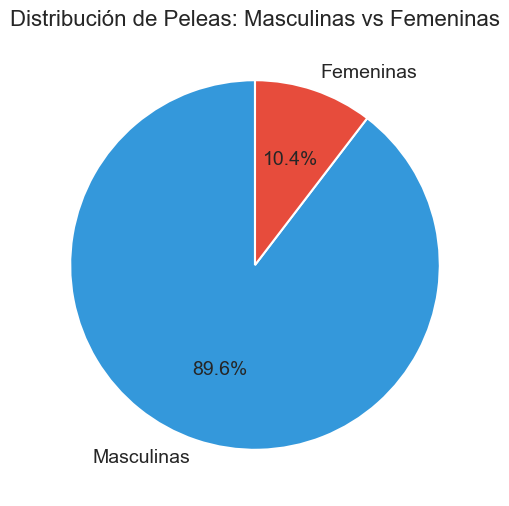
\includegraphics[width=0.6\textwidth]{DistribucionDePeleas.png}
    \caption{Distribución de peleas: Masculinas vs Femeninas.}
    \label{fig:peleas_dist}
\end{figure}

Debido a esta considerable diferencia en el volumen de registros, se decidió centrar el análisis y el desarrollo del modelo predictivo exclusivamente en las peleas masculinas. Esta medida busca evitar sesgos y asegurar que el análisis posterior se realice sobre un conjunto de datos homogéneo. A partir de este nuevo subconjunto, se procedió a evaluar la proporción de datos faltantes (ver Figura \ref{fig:cobertura_y_nulos}).

\begin{figure}[H]
    \centering
    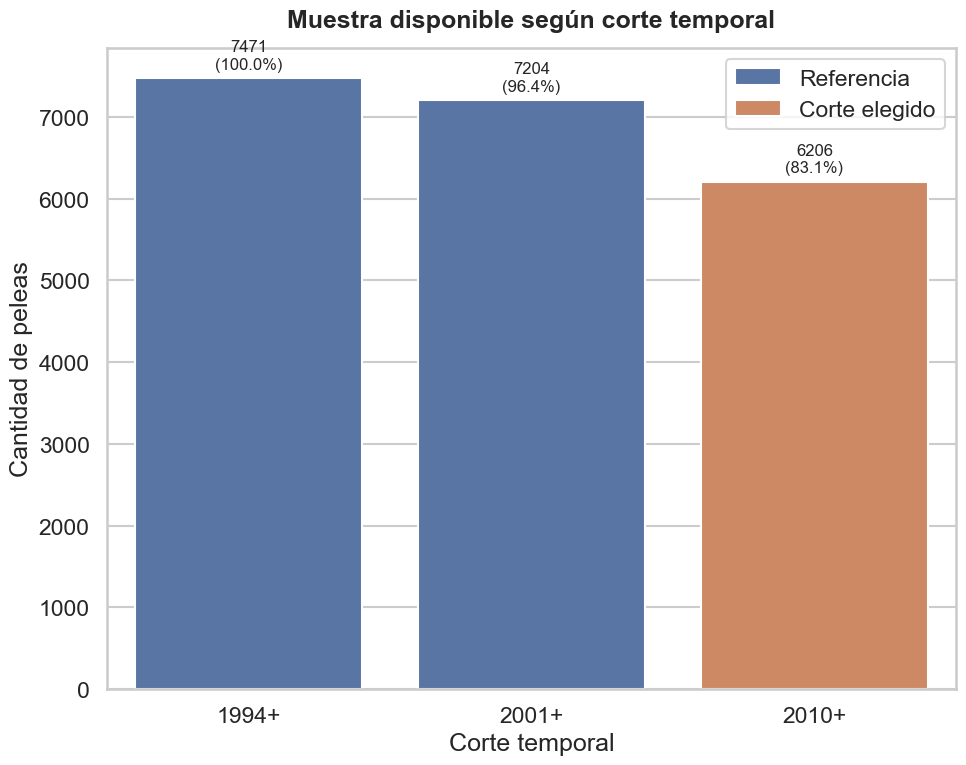
\includegraphics[width=0.85\textwidth]{CortePeleas.png}
    \caption{Cantidad de peleas conservadas según el corte temporal seleccionado.}
    \label{fig:corte-temporal-ufc}
\end{figure}

Otra consideración a tener en cuenta es el corte temporal. A partir de los objetivos del proyecto, se decidió concentrar el análisis principal en peleas desde 2010 en adelante. Este recorte temporal permite trabajar con una etapa más representativa de la UFC moderna, con reglas más estables, mayor profesionalización de los peleadores, divisiones más consolidadas y métricas técnicas más comparables. Las peleas anteriores pueden utilizarse como contexto histórico, pero no como base principal para entrenar modelos orientados a decisiones actuales.


También se evaluó la presencia de registros duplicados en el conjunto de datos. Al tratarse de un dataset histórico de eventos deportivos, la existencia de duplicados responde a errores en el proceso de recolección de datos o fallos en la carga de los mismos y no a circunstancias naturales del deporte. Sin embargo, \textbf{no se han encontrado duplicados} en el dataset. La manera en la que esto se confirmó fue buscando filas exactamente iguales, o peleas repetidas que quizás difieren por algún error de tipeo en otra columna (principalmente por fecha y peleadores). Ambas arrojaron cero coincidencias. 

\begin{figure}[H]
    \centering
    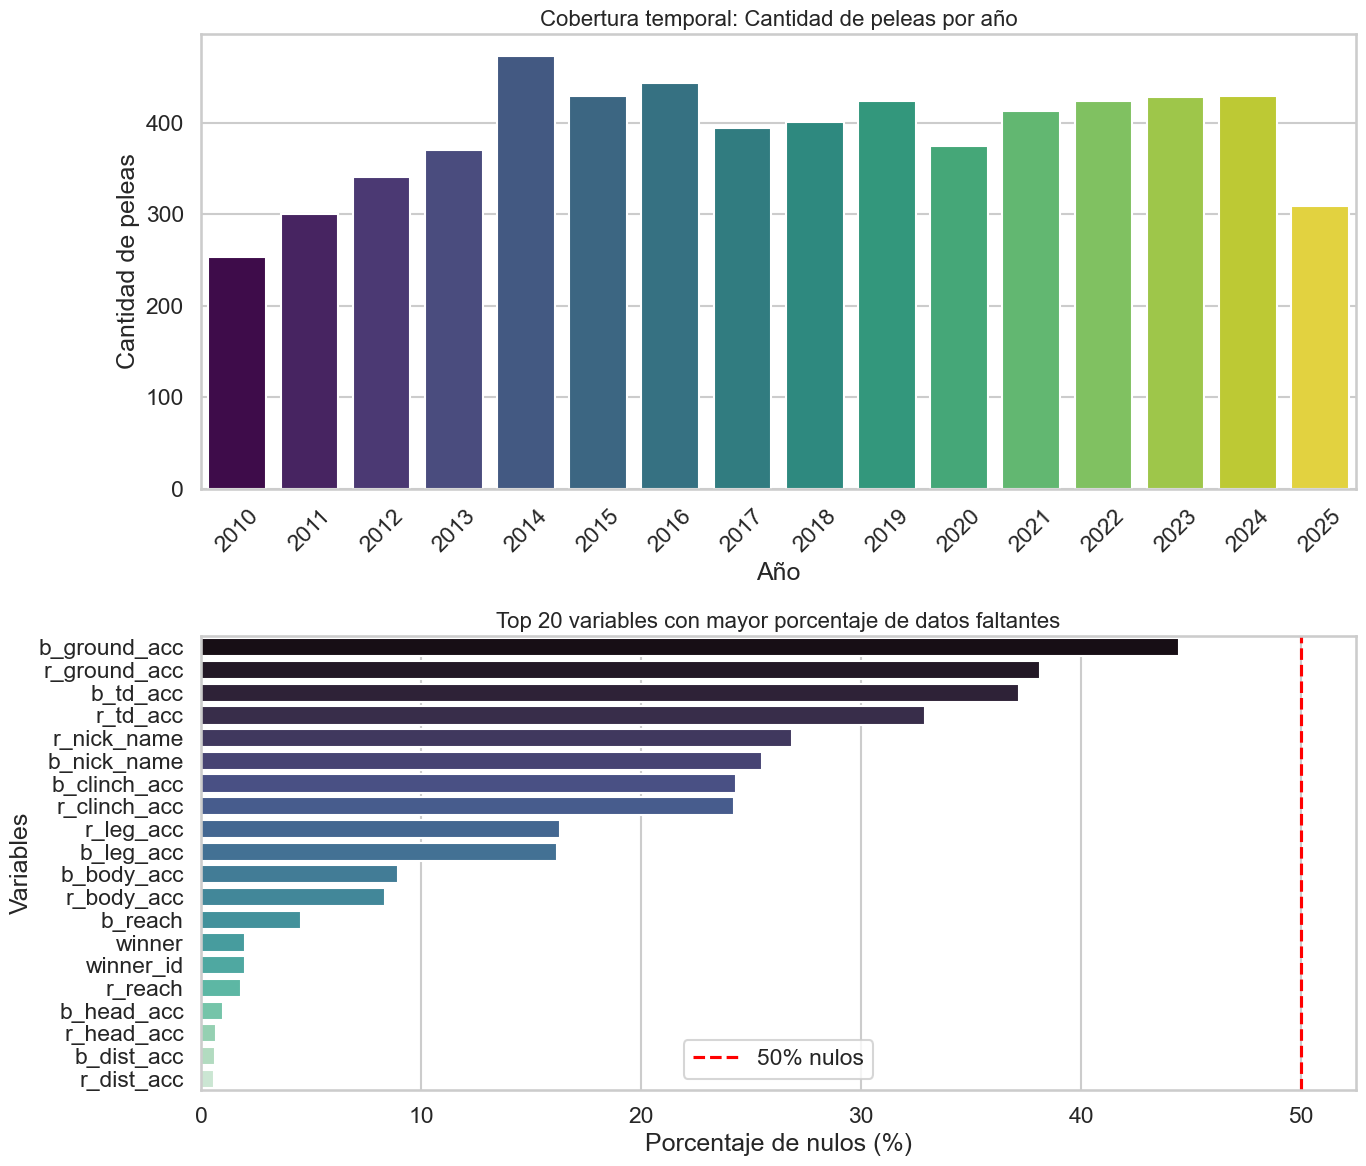
\includegraphics[width=1\textwidth]{DistribucionDeNulos.png}
    \caption{Cobertura temporal de las peleas por año (arriba) y análisis de atributos con mayor porcentaje de datos faltantes (abajo).}
    \label{fig:cobertura_y_nulos}
\end{figure}

Se aplicó un análisis visual mediante Boxplots para identificar valores atípicos en variables métricas fundamentales del combate, como la duración de la pelea y el volumen de golpes por minuto.

En lo que respecta a los outliers estadísticos (o casos excepcionales), hemos decidido poner el foco en métricas determinantes de un combate: duración y golpeo.
\begin{figure}[H]
    \centering
    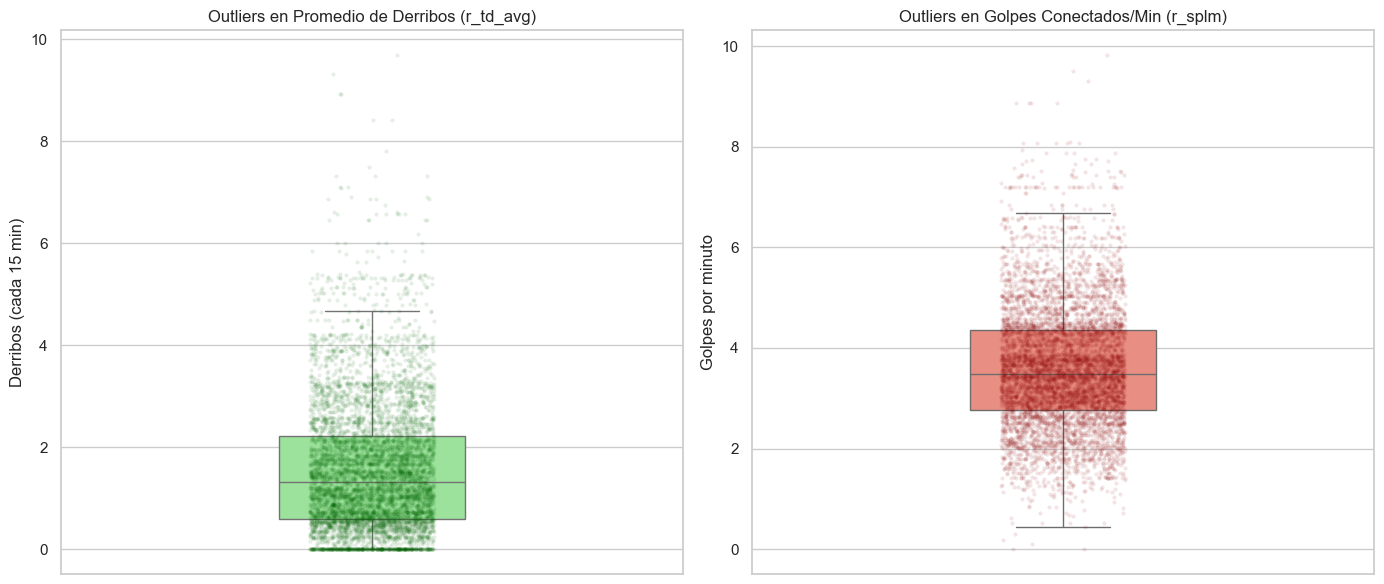
\includegraphics[width=1\textwidth]{outliers.png}
    \caption{Análisis visual para identificar valores atípicos en métricas del combate.}
    \label{fig:outliers}
\end{figure}

En el primero los valores atípicos inferiores corresponden a luchadores que basan su estrategia en llevar el combate al suelo repetidas veces. En las métricas de golpeo, los outliers superiores representan desempeños atléticos excepcionales (volumen de striking muy por encima de la media) y los inferiores los rendimientos menos deslumbrantes. Pero como estos outliers no pertenecen a errores de medición o carga (como lo sería un tiempo de pelea negativo), sino a eventos reales y posibles en el marco de un combate, se decide conservar la totalidad de los mismos. Eliminarlos implicaría sesgar el análisis, la capacidad de conectar muchos golpes o la incapacidad de ello son variables que un modelo debe incluir.

Otro análisis a tener en cuenta es la correlación entre los atributos. Observemos el siguiente gráfico:
\begin{figure}[H]
    \centering
    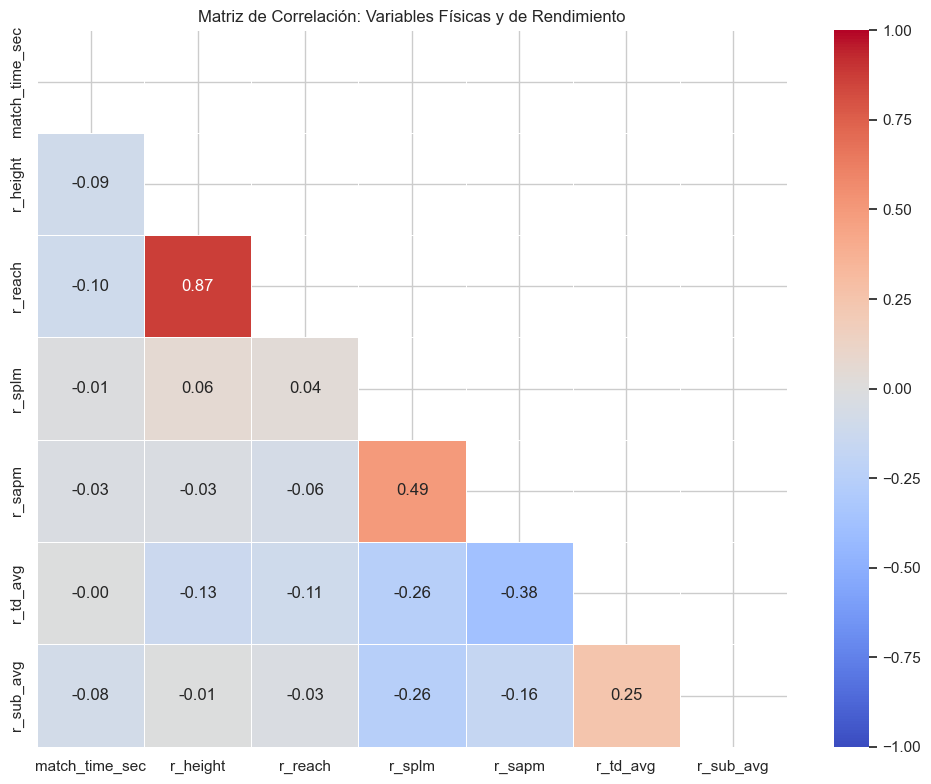
\includegraphics[width=1\textwidth]{heatmap.png}
    \caption{Matriz de Pearson para visualizar correlación entre las variables físicas y de rendimiento deportivo.}
    \label{fig:heatmap}
\end{figure}
Algunos puntos a destacar son la fuerte correlación positiva (0.87) entre la altura y la envergadura, lo cual es esperable ya que las personas altas suelen tener brazos más largos; la correlación moderada de (0.49) entre los golpes conectados y recibidos, indicando que los peleadores con estrategias muy ofensivas tienden a exponerse a más golpes.

Si bien la depuración definitiva se llevará a cabo tras un análisis exploratorio más profundo, se estableció un criterio preliminar para el manejo de los valores nulos y la selección de variables. Este enfoque está orientado específicamente a responder las tres preguntas centrales de este trabajo. Pero, por ahora, ¿cuál es la calidad de este dataset? Observemos el siguiente gráfico.

\begin{figure}[H]
    \centering
    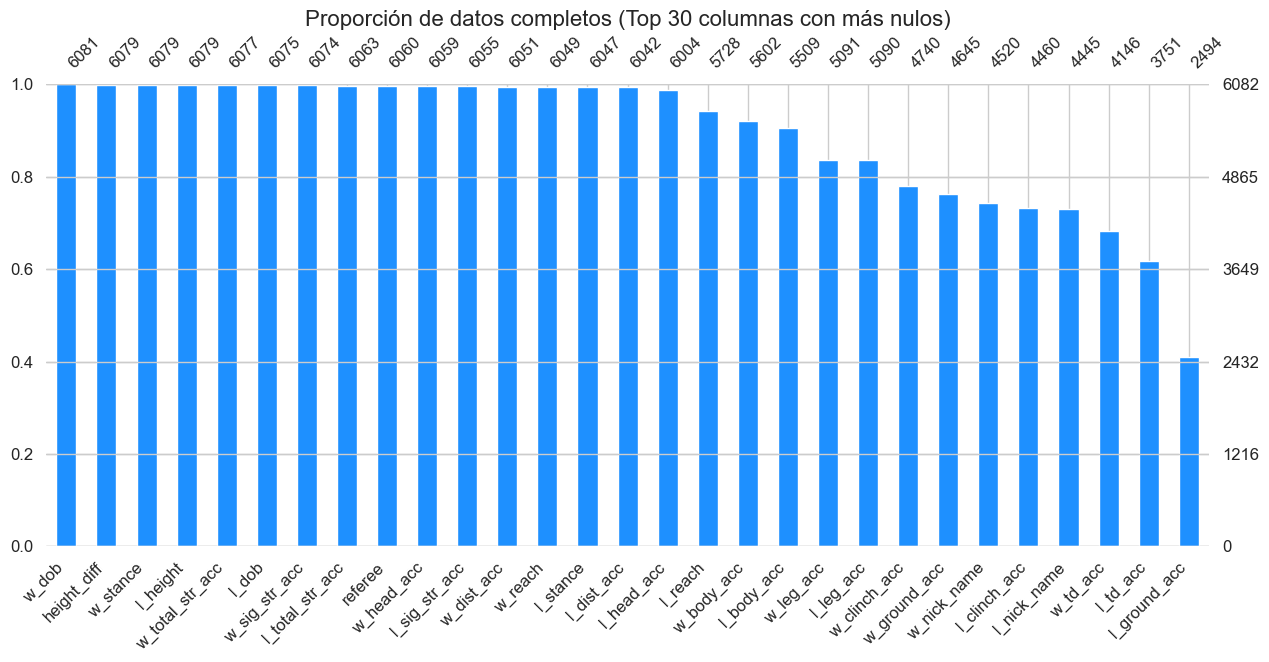
\includegraphics[width=0.95\textwidth]{DatosFaltantes.png}
    \caption{Proporción de datos completos en las 30 columnas con mayor cantidad de valores faltantes para peleas masculinas de UFC desde 2010.}
    \label{fig:datos-faltantes}
\end{figure}

\noindent
El gráfico evidencia que el dataset presenta una buena completitud general en variables físicas y biográficas, pero mayores faltantes en métricas técnicas específicas del combate. Esto permite distinguir entre variables aptas para un análisis pre-pelea, como edad, altura, alcance o postura, y variables que deben tratarse con precaución o excluirse, como estadísticas generadas durante la pelea. 

Antes de avanzar con el modelado, es fundamental comprender la dinámica estructural de los enfrentamientos. Como se observa en la Figura \ref{fig:estructura_combate}, se exploraron cuatro métricas contextuales clave: la cantidad de peleas por división de peso, los métodos de finalización del combate, la distribución de los rounds de cierre y la duración total en minutos. Este resumen descriptivo permite vislumbrar cómo tienden a resolverse los encuentros según el peso y el tiempo.

\begin{figure}[H]
    \centering
    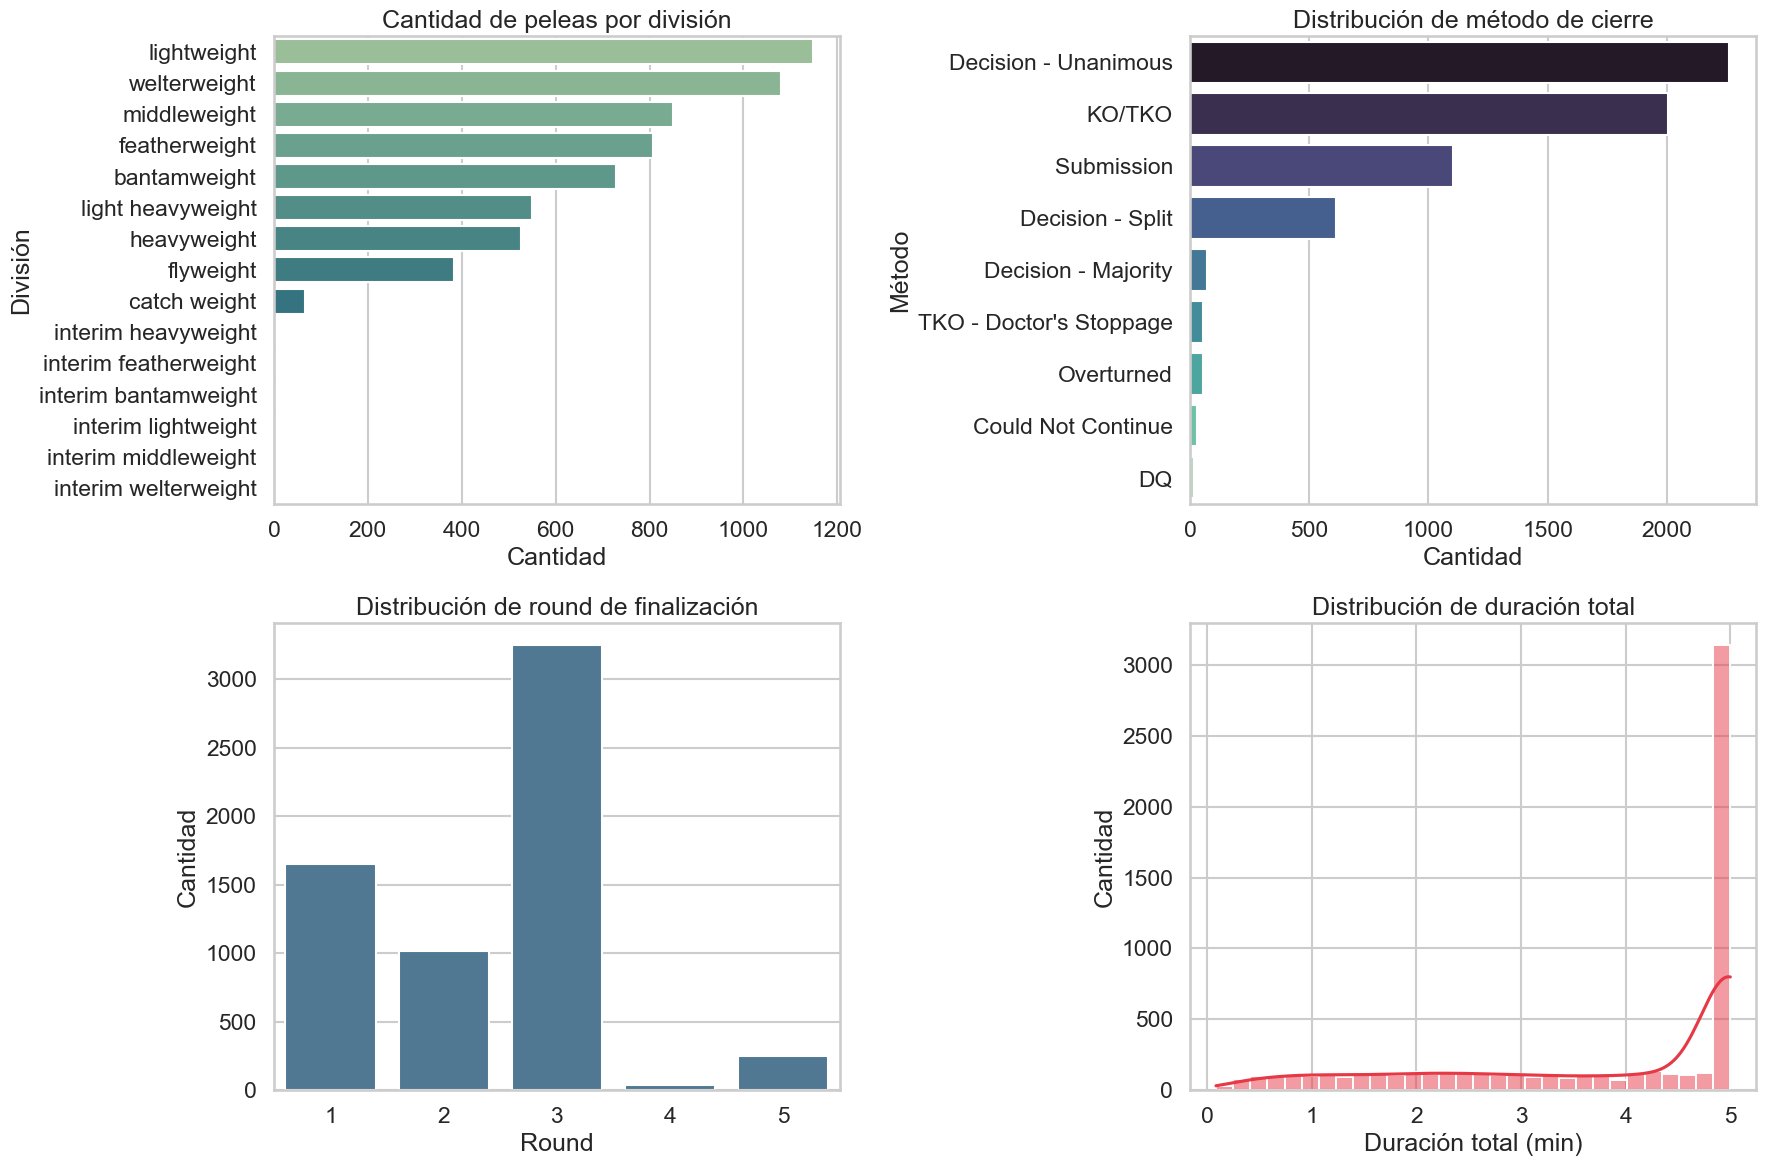
\includegraphics[width=1\textwidth]{Imagen3.png}
    \caption{Análisis exploratorio: cantidad de peleas por división, método de cierre, round de finalización y duración de los combates.}
    \label{fig:estructura_combate}
\end{figure}

\begin{figure}[H]
    \centering
    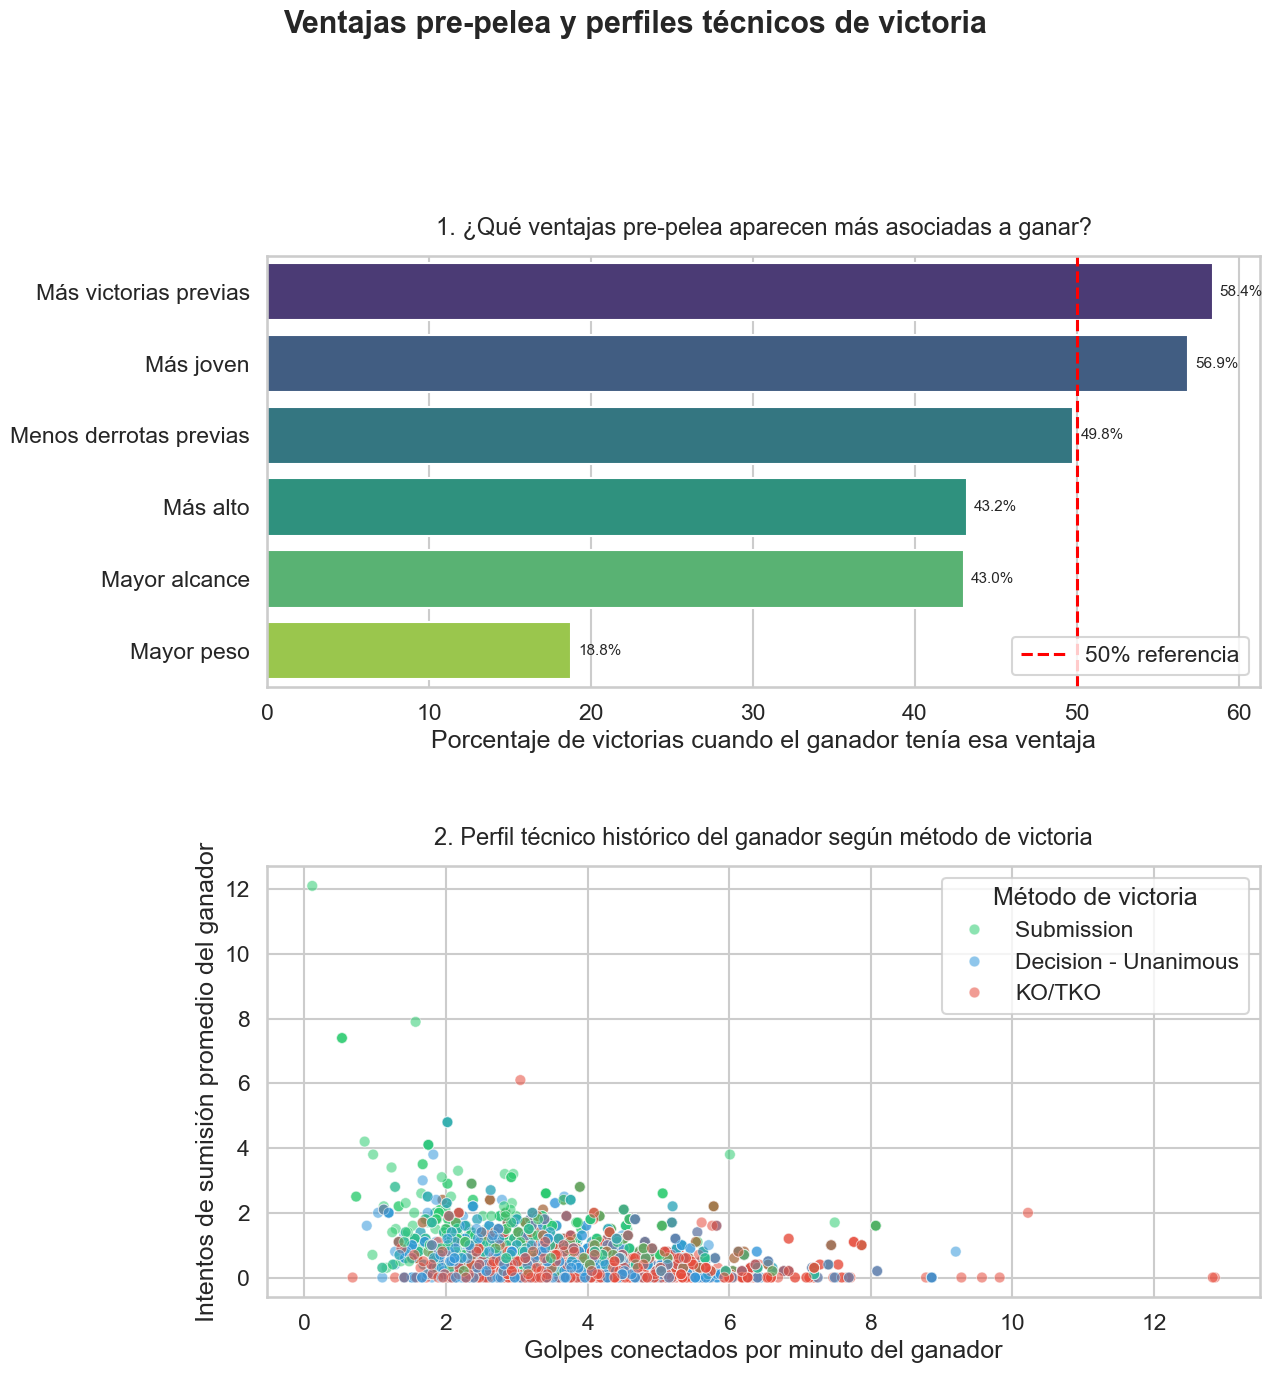
\includegraphics[width=0.95\textwidth]{VentajasPerfilesVictoria.png}
    \caption{Ventajas pre-pelea y perfiles técnicos asociados a los métodos de victoria en peleas masculinas de UFC desde 2010.}
    \label{fig:ventajas-perfiles-ufc}
\end{figure}

\noindent
El primer gráfico analiza variables disponibles antes de la pelea, evitando utilizar métricas generadas durante el combate, como golpes conectados o derribos concretados. Esta decisión es importante porque el objetivo del trabajo es aproximarse a una predicción previa del resultado, no explicar el resultado una vez ocurrida la pelea. En ese sentido, variables como edad, altura, alcance, peso y récord previo son más adecuadas para un enfoque predictivo.

\vspace{0.3cm}

\noindent
A partir del gráfico se puede observar que las ventajas físicas o de trayectoria previa presentan asociaciones moderadas con la victoria, pero ninguna de ellas determina por sí sola el resultado. Esto sugiere que ganar una pelea no depende únicamente de una característica aislada, sino de la combinación entre características físicas, experiencia, estilo técnico, emparejamiento y contexto competitivo.

\vspace{0.3cm}

\noindent
El segundo gráfico cruza dos dimensiones técnicas históricas del ganador: volumen de golpeo e intentos promedio de sumisión. La superposición entre métodos de victoria indica que los estilos no aparecen completamente separados. Aunque los ganadores por KO/TKO tienden a relacionarse más con el volumen de striking y los ganadores por sumisión con mayor actividad grappler, existen muchos casos intermedios. Esto refuerza la idea de que los perfiles modernos de UFC son híbridos y que un modelo predictivo debería combinar múltiples variables técnicas, físicas y contextuales.

Para complementar esta visión estática de los combates, se analizó también la progresión histórica de estas métricas. La Figura \ref{fig:evolucion_metodos_duracion} refleja la evolución temporal de los métodos de finalización y la duración promedio, evidenciando cómo han cambiado las tendencias de resolución (decisiones, nocauts y sumisiones) a lo largo de los años en la franquicia.

\begin{figure}[H]
    \centering
    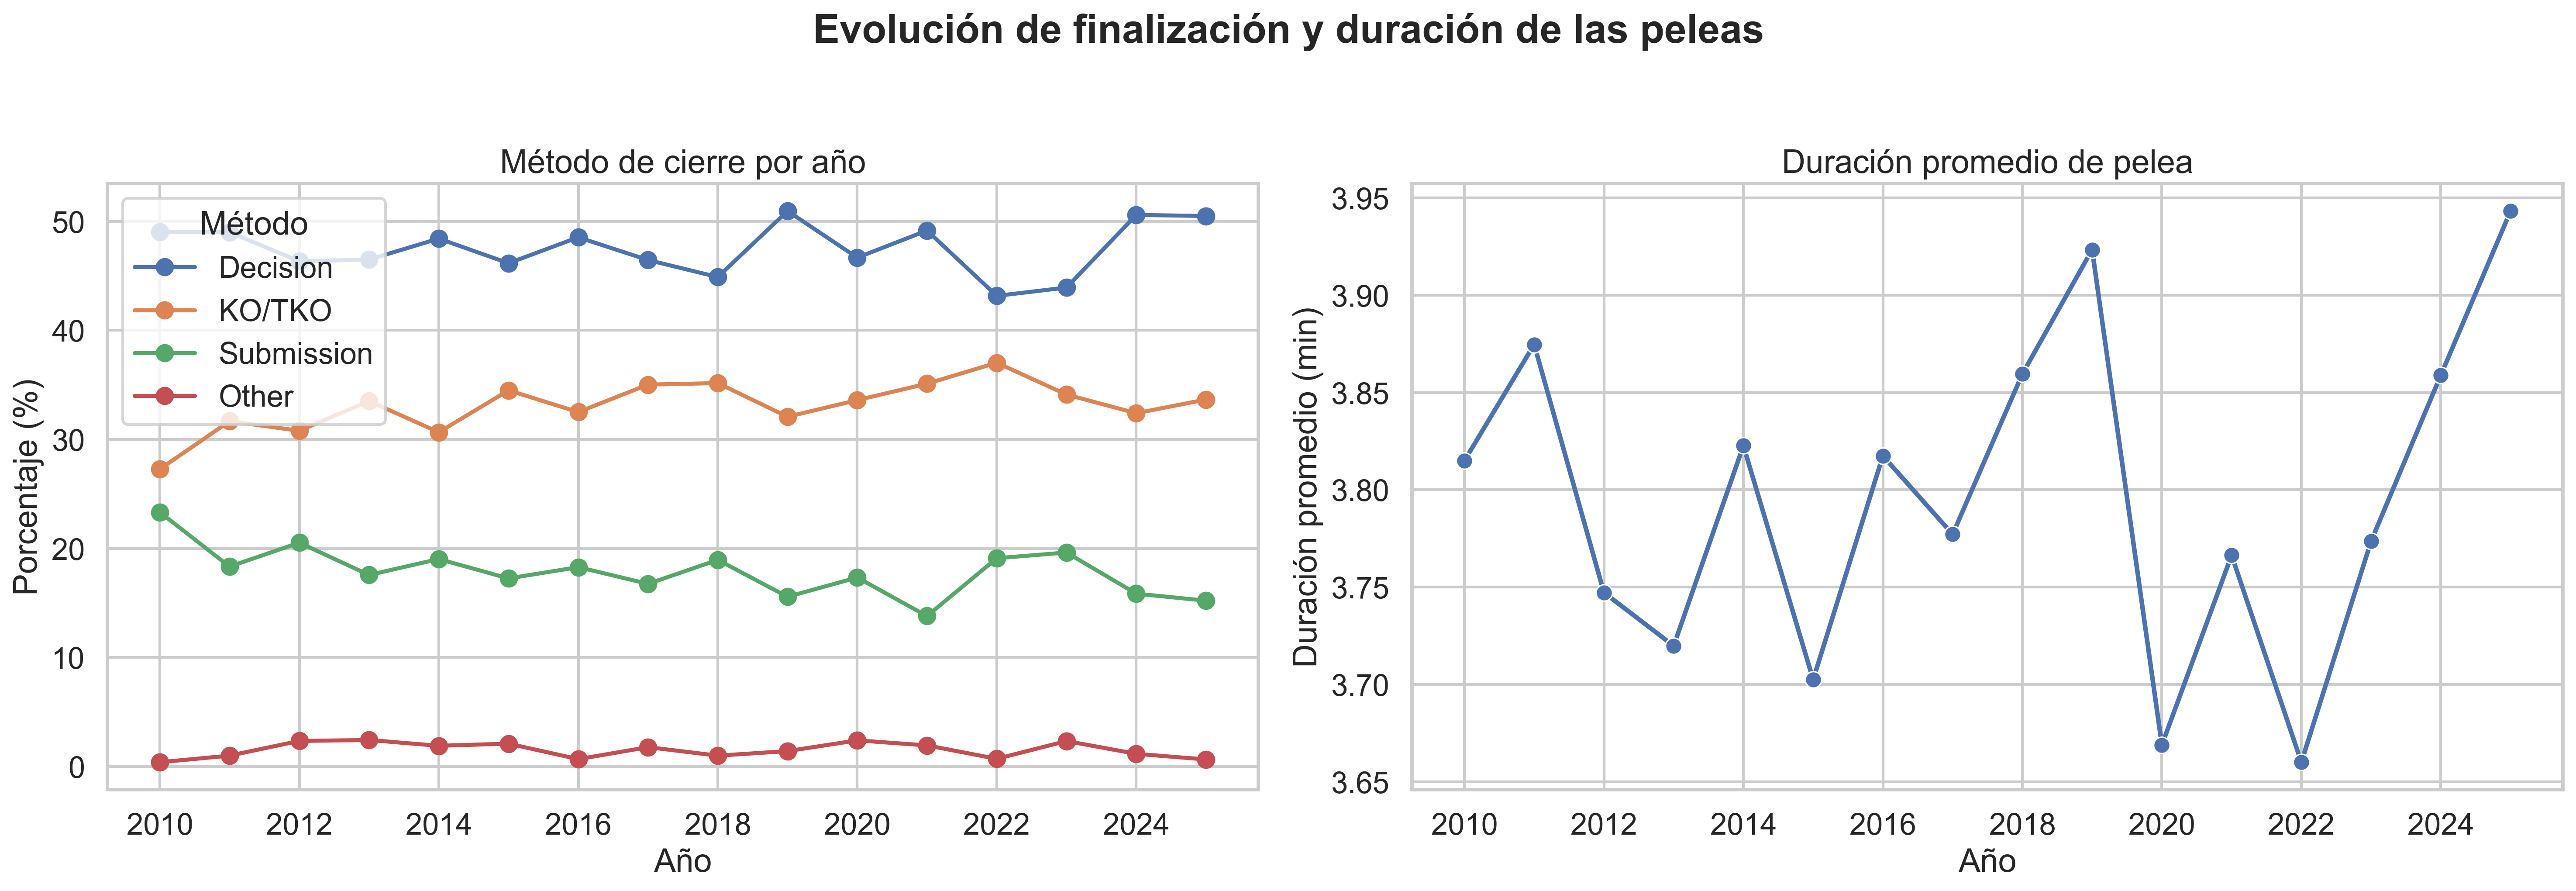
\includegraphics[width=1\textwidth]{Evolucion_Metodos_Duracion.png}
    \caption{Evolución temporal de los métodos de finalización y de la duración promedio de los combates. Se muestra la variación en la proporción de decisiones, nocauts y sumisiones a lo largo del tiempo, junto con la duración media de las peleas por año.}
    \label{fig:evolucion_metodos_duracion}
\end{figure}

Finalmente, la Figura \ref{fig:evolucion_tecnica} expone la evolución competitiva y técnica general de la UFC. Allí se contrasta el porcentaje de peleas por el título respecto al total, junto con variaciones en métricas de combate fundamentales, tanto de \textit{striking} (golpes conectados y recibidos por minuto) como de \textit{grappling} (derribos y sumisiones promedio).

\begin{figure}[H]
    \centering
    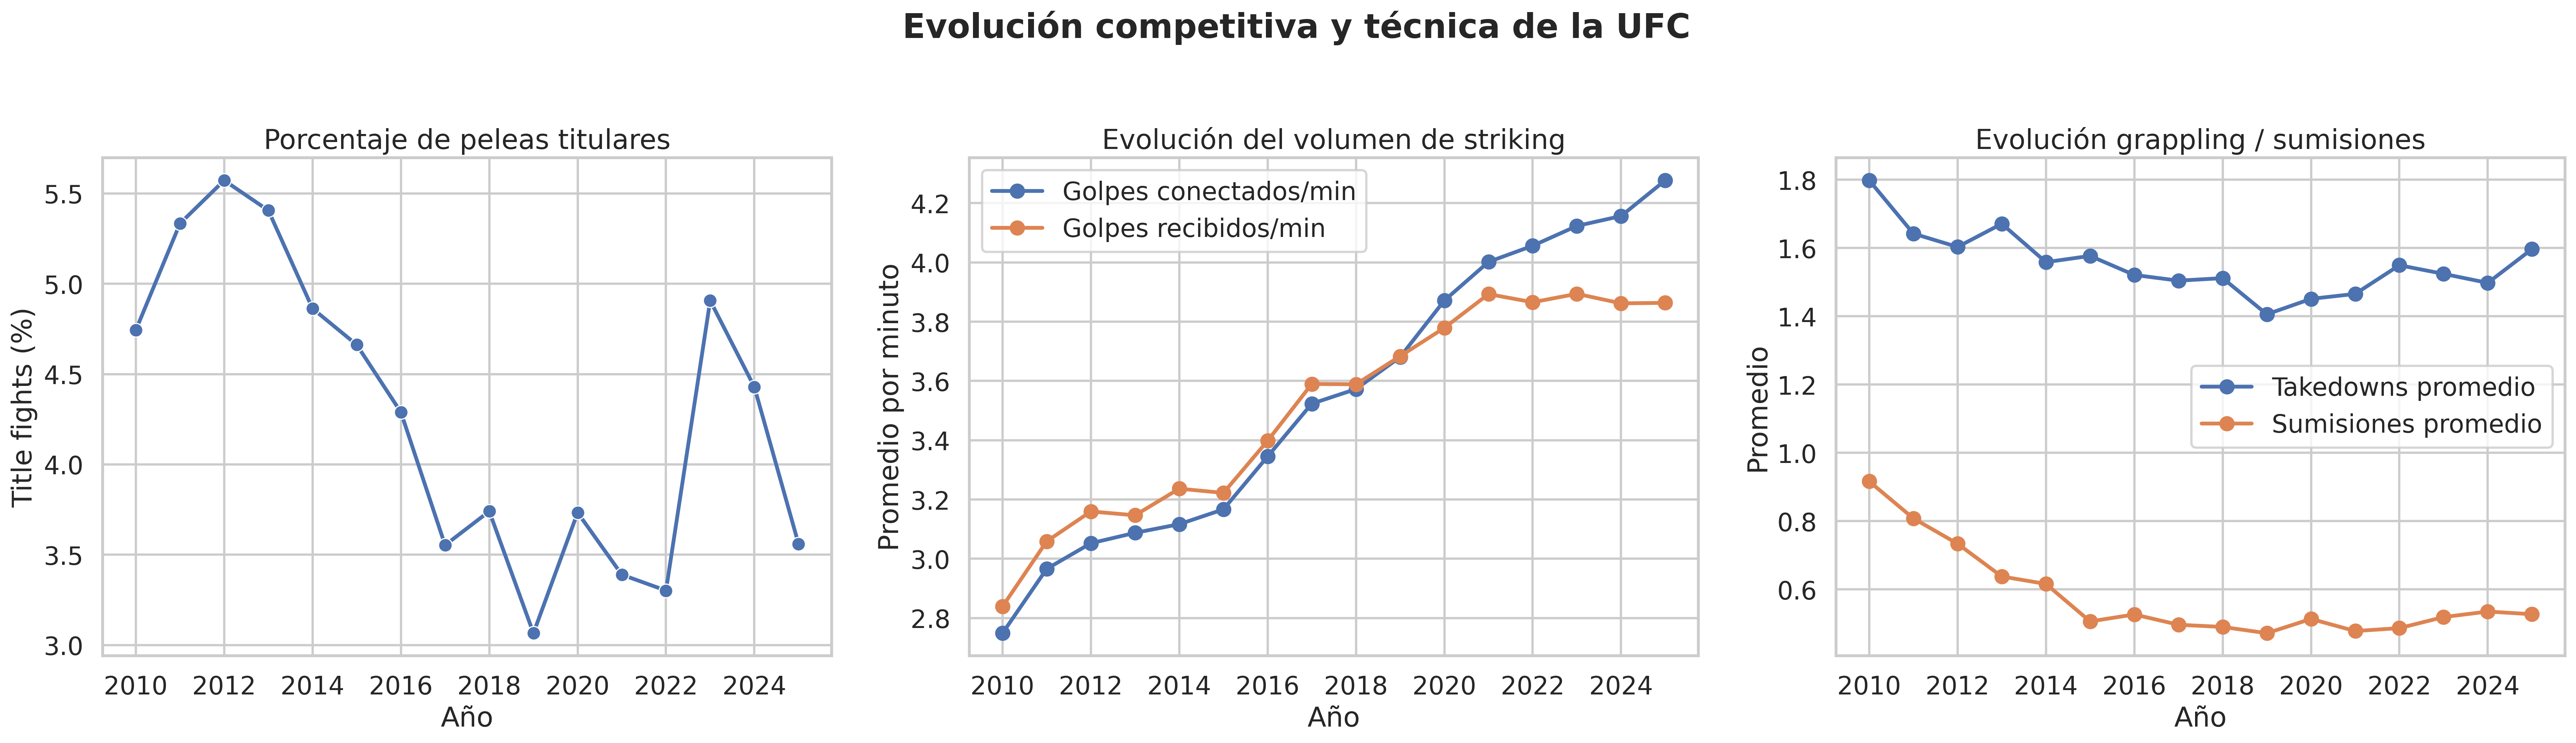
\includegraphics[width=1\textwidth]{Evolucion_Tecnica.png}
    \caption{Evolución competitiva y técnica de la UFC. Se presenta el porcentaje de peleas titulares por año junto con la evolución de métricas de striking (golpes conectados y recibidos por minuto) y grappling (derribos y sumisiones promedio).}
    \label{fig:evolucion_tecnica}
\end{figure}

Para darle un cierre a esta etapa de análisis, se aplicó un modelo de aprendizaje no supervisado (K-medias) sobre múltiples atributos técnicos para identificar estilos de combate. Se utilizaron las variables: golpes conectados por minuto, precisión de golpeo, golpes recibidos, defensa de golpeo, promedio de derribos, precisión de derribo, defensa de derribo y promedio de sumisiones, todas estandarizadas previamente.

\begin{figure}[H]
    \centering
    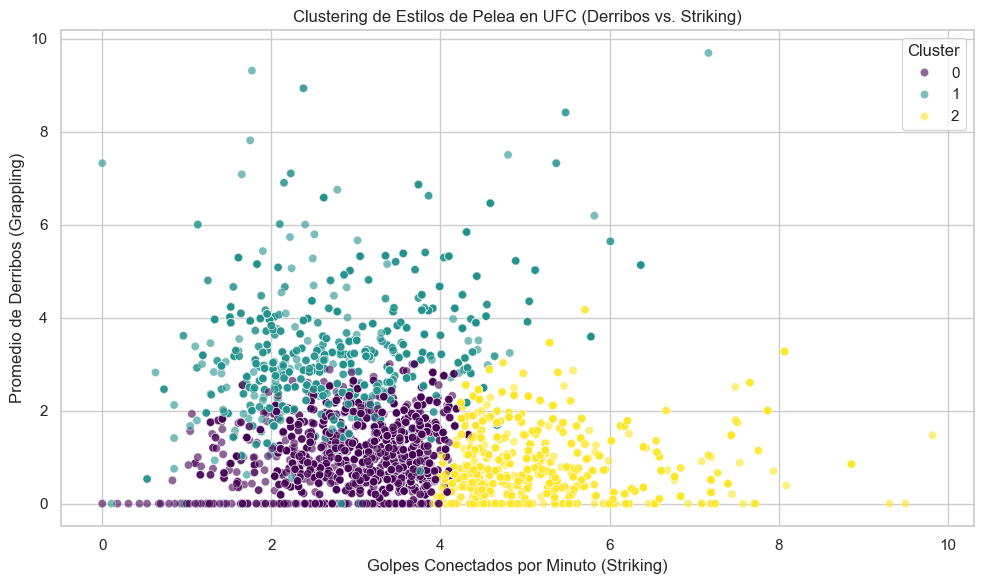
\includegraphics[width=1\textwidth]{clustering.png}
    \caption{Separación de perfiles clásicos del MMA mediante Clustering por K-Medias.}
    \label{fig:clustering}
\end{figure}

Para justificar la elección de $k=3$, se aplicaron el método del codo y el cálculo de silhouette. El gráfico del codo mostró una inflexión clara en $k=3$, y el silhouette también confirmó que este valor ofrece la mejor separación entre grupos.

\begin{figure}[H]
    \centering
    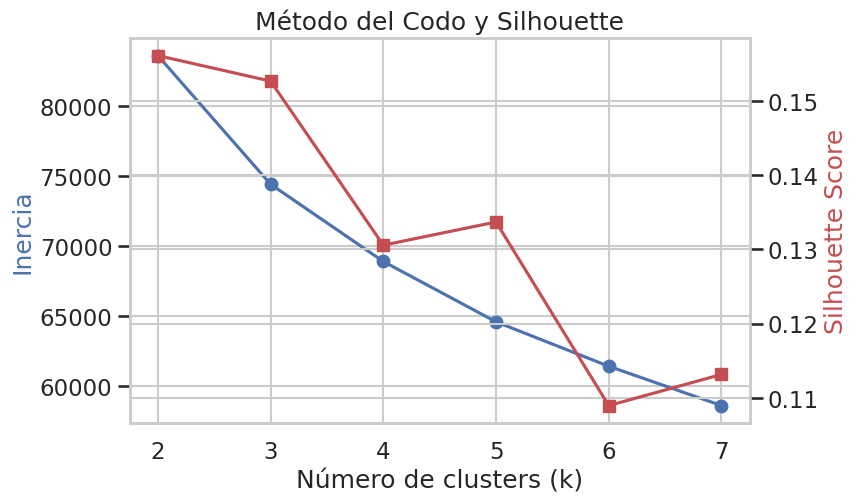
\includegraphics[width=1\textwidth]{codo_y_silouette.png}
    \caption{Método del codo y Silhouette graficados.}
    \label{fig:codo-silhouette}
\end{figure}

Al segmentar la población en 3 clusters, se lograron diferenciar tres arquetipos, los cuales se describen a partir de sus centroides (ver Tabla \ref{tab:centroides}):

\begin{table}[H]
    \centering
    \footnotesize
    \setlength{\tabcolsep}{3.5pt}
    \begin{tabular}{ccccccccc}
        \toprule
        \textbf{Cluster} & \textbf{splm} & \textbf{str\_acc (\%)} & \textbf{sapm} & \textbf{str\_def (\%)} & \textbf{td\_avg} & \textbf{td\_acc (\%)} & \textbf{td\_def (\%)} & \textbf{sub\_avg} \\
        \midrule
        0 & 4.53 & 45.99 & 4.28 & 53.96 & 0.81 & 31.34 & 69.52 & 0.28 \\
        1 & 3.11 & 45.86 & 2.74 & 57.14 & 2.40 & 47.01 & 66.64 & 0.57 \\
        2 & 2.62 & 41.92 & 3.55 & 48.88 & 1.40 & 28.52 & 38.55 & 1.09 \\
        \bottomrule
    \end{tabular}
    \caption{Valores de los centroides en la escala original para cada cluster.}
    \label{tab:centroides}
\end{table}

\begin{itemize}
    \item \textbf{Cluster 0 (Estilo Mixto):} Agrupa a peleadores con métricas intermedias y equilibradas. Conectan alrededor de 4.5 golpes por minuto y tienen un promedio de derribos moderado, representando a luchadores todoterreno.
    \item \textbf{Cluster 1 (Strikers):} Atletas con alto volumen de golpes y buena precisión, que reciben menos daño (sapm bajo) y muestran buena defensa de derribo, pero sus intentos de llevar la pelea al suelo y buscar sumisiones son casi nulos.
    \item \textbf{Cluster 2 (Grapplers):} Competidores con una alta tasa de derribos y control en el suelo, con el mayor promedio de sumisiones (sub\_avg alto), pero que conectan menor cantidad de golpes y muestran la menor precisión de golpeo.
\end{itemize}

El conjunto de datos resultante es sólido, no tiene redundancias críticas y define estilos de pelea de forma precisa. Esto lo deja en condiciones ideales para implementar modelos predictivos.

%A continuación, se detalla el enfoque proyectado para cada una de las preguntas de investigación:

%\subsection*{1. ¿Qué luchador tiene mayor probabilidad de ganar una pelea dada?}
%Dado que este problema se abordará como una tarea de clasificación binaria, es de vital importancia utilizar únicamente información disponible \textbf{antes} de que ocurra el combate. 

%Por lo tanto, se descartarán todas las estadísticas recolectadas \textit{durante} la pelea en sí (tales como la cantidad de golpes conectados en un round específico, tiempos de control y porcentajes de precisión). Las variables a conservar incluyen metadatos del evento (división, si es por el título, cantidad de rounds) y características pre-combate de cada peleador (récord de victorias/derrotas, postura, edad calculada a partir de la fecha de nacimiento y atributos físicos). 

%Los valores faltantes en estas variables retenidas se imputarán empleando sus respectivas modas o medianas segmentadas por división. Finalmente, se filtrarán estrictamente las peleas sin un ganador definido para poder entrenar adecuadamente el modelo clasificador (ej. Regresión Logística o Random Forest).

%\subsection*{2. Si soy un luchador con determinadas características, ¿qué tipo de pelea me conviene aceptar?}
%En este escenario, el objetivo es recomendar el contexto de pelea que maximice la probabilidad de victoria. 
%Se mantendrán las características físicas y de historial del luchador (previamente imputadas), centrando el análisis en las variables de contexto: cantidad de rounds pactados, división, si hay un título en juego y el referí. 

%Para variables de contexto con datos faltantes (por ejemplo, la cantidad de rounds), se realizará una imputación basada en la naturaleza del combate (utilizando la variable \textit{title\_fight} como pista, ya que estas suelen ser a 5 rounds). En el caso de valores ausentes en el campo del árbitro, se generará una categoría independiente (\textit{Unknown}). Se construirá un modelo que prediga la probabilidad de ganar en función de las características fijas del luchador interactuando con las distintas combinaciones posibles del contexto de pelea.

%\subsection*{3. Si soy una persona con determinadas características, ¿qué estilo me conviene practicar?}
%Esta pregunta requiere cambiar el nivel de análisis: de un enfoque por combate individual a un perfil agregado por luchador. 
%Para determinar un estilo de pelea (por ejemplo, \textit{Striker} puro, \textit{Grappler} o \textit{Balanceado}), se utilizarán estadísticas históricas acumuladas de cada combatiente (promedio de golpes significativos, derribos y sumisiones). 

%Al crear este nuevo dataset agrupado por luchador, aquellos registros mínimos que presenten valores nulos en columnas esenciales de golpes (como \textit{sig\_str\_landed}) podrán ser directamente eliminados sin impacto significativo (representan menos del 1\% del conjunto). Una vez consolidada la base limpia, se aplicarán algoritmos de agrupamiento (ej. \textit{K-Means}) sobre las estadísticas ofensivas para asignar un estilo definitivo a cada peleador. La recomendación final consistirá en buscar en este espacio a los luchadores físicamente más similares a la persona consultante que posean un porcentaje de victorias superior al 50\%, recomendando el estilo predominante de este subgrupo exitoso.


\section{Análisis Predictivo Pre-Pelea y Respuesta a las Preguntas}

Se entrenaron un clasificador Naïve Bayes Gaussiano y un Árbol de Decisión (criterio entropía, profundidad máxima de 5) utilizando únicamente variables pre-pelea: diferencias de edad, altura, alcance, victorias, derrotas y defensa de golpeo (diff\_str\_def). 

Para evaluar estos modelos, se definió un modelo base (baseline). El conjunto de prueba contiene 1217 combates, donde 711 son victorias del rincón rojo y 506 del rincón azul. Por tanto, predecir siempre que ganará el rincón rojo arroja una precisión base del 58,42\%.

El Árbol de Decisión logró una exactitud del 65,74\% en el conjunto de prueba, lo que demuestra una mejora de más de 7 puntos porcentuales con respecto a la predicción estática (baseline). Además, el algoritmo tiene una dificultad de cómputo en la fase de entrenamiento de $\mathcal{O}(n \cdot d \log(n))$, donde $n$ es la cantidad de muestras y $d$ la de atributos, y de $\mathcal{O}(\text{profundidad})$ en la predicción. En el dominio de las MMA, esto es sumamente útil porque permite evaluar ventajas en tiempo real de forma instantánea.

Las métricas detalladas por clase para el Árbol de Decisión muestran el siguiente comportamiento:

\textbf{En Entrenamiento:}
\begin{itemize}
    \item \textbf{Precisión (Precision):} 64\% general. Ayuda a confiar en que la predicción de victoria de un luchador es segura y no una falsa alarma. Útil para estrategias de apuestas y selección de peleas.
    \item \textbf{Recall:} 65\% para la clase Azul y 63\% para la clase Roja. Indica qué proporción de las victorias reales logra encontrar el modelo. Crucial para no perder de vista oportunidades reales de victoria.
    \item \textbf{F1-Score:} 65\% para la Azul y 64\% para la Roja. Brinda un balance entre precisión y recall, ideal porque en MMA los falsos positivos y falsos negativos tienen costos estratégicos diferentes.
\end{itemize}
La matriz de confusión en entrenamiento arrojó 3209 verdaderos negativos, 1696 falsos positivos, 1770 falsos negativos y 3056 verdaderos positivos.

\textbf{En Prueba:}
\begin{itemize}
    \item \textbf{Precisión (Precision):} 61\% para la clase Azul y 64\% para la clase Roja. 
    \item \textbf{Recall:} 63\% para la Azul y 62\% para la Roja.
    \item \textbf{F1-Score:} 62\% para la Azul y 63\% para la Roja.
\end{itemize}
La matriz de confusión en prueba evidenció 739 verdaderos negativos, 438 falsos positivos, 479 falsos negativos y 777 verdaderos positivos.

El árbol de clasificación, a pesar de su menor recall para la clase minoritaria, permite extraer reglas interpretables. Tras analizar su estructura (Figura~\ref{fig:arbol_pre_pelea}) se observa que la primera división suele estar basada en \texttt{diff\_str\_def <= -11.5}, lo que indica que si el luchador azul tiene una defensa de golpeo muy superior a la del rojo, el árbol predice victoria del azul. En caso contrario, se evalúan diferencias en victorias acumuladas y edad. 

\subsection{¿Qué luchador tiene mayor probabilidad de ganar?}
Para una pelea dada, se calculan las diferencias (rojo - azul) y se recorre el árbol hasta una hoja. La clase mayoritaria de esa hoja indica el luchador con mayor probabilidad. Por ejemplo, si \texttt{diff\_wins > -0.5} y \texttt{diff\_age <= 2.0}, el árbol predice \textit{Gana Rojo}. El modelo Naïve Bayes complementa entregando una probabilidad concreta $P(\text{gana rojo} \mid \text{diferencias})$, permitiendo comparar la confianza de la predicción.

\subsection{¿Qué tipo de pelea me conviene aceptar?}
Fijando mis propias características (edad, victorias, derrotas, defensa de golpeo), puedo variar los atributos del oponente y observar qué ramas del árbol conducen a mi victoria. De las reglas se deduce:
\begin{itemize}
    \item \textbf{Me conviene aceptar peleas contra oponentes con peor defensa de golpeo} (que mi \texttt{diff\_str\_def} sea positivo y alto).
    \item \textbf{Me conviene que mi oponente tenga menos victorias y más derrotas} (diferencias favorables).
    \item \textbf{Si soy más joven}, la ventaja es mayor.
\end{itemize}
Por tanto, el árbol proporciona umbrales concretos: por ejemplo, si \texttt{diff\_str\_def > -11.5} y \texttt{diff\_wins > -0.5}, entonces aceptar la pelea es favorable si además soy más joven.

\subsection{¿Qué estilo me conviene practicar?}
Dado que el árbol incluye \texttt{diff\_str\_def} (defensa de golpeo), se infiere que mejorar la defensa de golpeo es un factor relevante para aumentar la probabilidad de victoria. Si un luchador tiene baja defensa, debería practicar un estilo que minimice los golpes recibidos (por ejemplo, lucha en el suelo o clinch). Por el contrario, si tiene alta defensa, puede destacar en striking. La edad y el récord también orientan: un luchador joven puede permitirse un estilo más agresivo; un veterano debería priorizar la defensa y la experiencia.

\subsection{¿Conviene un árbol de mayor profundidad?}
Se probaron distintas profundidades máximas. El árbol actual (con poda para evitar sobreajuste) tiene una profundidad de 4-5 niveles. Aumentar la profundidad produce reglas más específicas pero reduce la exactitud en prueba (validación cruzada mostró descenso del 66\% al 63\% con profundidad >7). Por tanto, la profundidad actual es adecuada para equilibrar sesgo y varianza.

\begin{figure}[H]
    \centering
    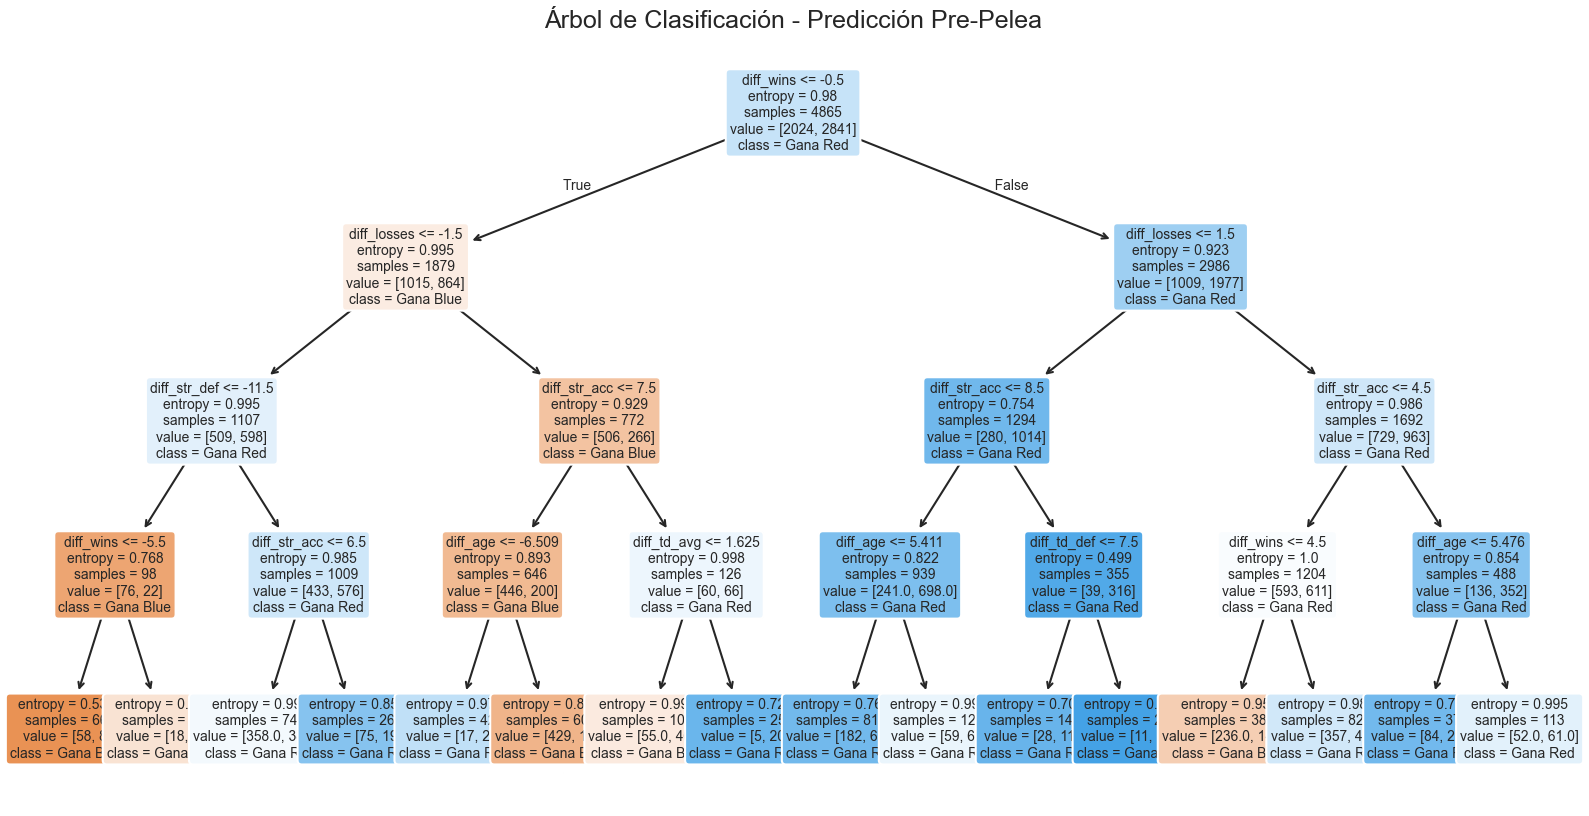
\includegraphics[width=0.9\textwidth]{ArboldeClasificacion-PrediccionPrePelea.png}
    \caption{Árbol de clasificación pre-pelea. Las ramas principales involucran \texttt{diff\_str\_def}, \texttt{diff\_wins} y \texttt{diff\_age}.}
    \label{fig:arbol_pre_pelea}
\end{figure}

\end{document}